% --- LaTeX Dokument ------------------------------------------------------
% Dokument für Ausarbeitung im Fach Komponentenbasierte Softwareentwicklung
% ------------------------------------------------------------------------

% Dokumentenklasse (Koma Script) -----------------------------------------
\documentclass[%
   final,      % fertiges Dokument
   paper=a4, paper=portrait, pagesize=auto, % Papier Einstellungen
   fontsize=11pt, % Schriftgröße
   ngerman, % Sprache 
 ]{scrartcl} % Classes: scrartcl, scrreprt, scrbook

% ~~~~~~~~~~~~~~~~~~~~~~~~~~~~~~~~~~~~~~~~~~~~~~~~~~~~~~~~~~~~~~~~~~~~~~~~
% encoding

% Encoding der Dateien (sonst funktionieren Umlaute nicht)
\usepackage[utf8]{inputenc}
%\usepackage{wasysym}
% Encoding der Verzeichnisse (für Pfade mit Umlauten und Leerzeichne)
\usepackage[%
   extendedchars, encoding, multidot, space,
   % filenameencoding=latin1, % Windows XP, Vista, 7
   filenameencoding=utf8,   % Linux, OS X
]{grffile}

% ~~~~~~~~~~~~~~~~~~~~~~~~~~~~~~~~~~~~~~~~~~~~~~~~~~~~~~~~~~~~~~~~~~~~~~~~
% Pakete und Stile
% ~~~~~~~~~~~~~~~~~~~~~~~~~~~~~~~~~~~~~~~~~~~~~~~~~~~~~~~~~~~~~~~~~~~~~~~~
% Schriften
% ~~~~~~~~~~~~~~~~~~~~~~~~~~~~~~~~~~~~~~~~~~~~~~~~~~~~~~~~~~~~~~~~~~~~~~~~
% Fonts Fonts Fonts
% ~~~~~~~~~~~~~~~~~~~~~~~~~~~~~~~~~~~~~~~~~~~~~~~~~~~~~~~~~~~~~~~~~~~~~~~~

% immer laden:
\usepackage[T1]{fontenc} % T1 Schrift Encoding
\usepackage{textcomp}	 % Zusätzliche Symbole (Text Companion font extension)

% ~~~~~~~~~~~~~~~~~~~~~~~~~~~~~~~~~~~~~~~~~~~~~~~~~~~~~~~~~~~~~~~~~~~~~~~~
% Symbole
% ~~~~~~~~~~~~~~~~~~~~~~~~~~~~~~~~~~~~~~~~~~~~~~~~~~~~~~~~~~~~~~~~~~~~~~~~

\usepackage{amssymb}
\usepackage{mathcomp}


%% ==== Zusammengesetzte Schriften  (Sans + Serif) =======================

%% - Latin Modern
\usepackage{lmodern}
%% -------------------

%% - Bera Schriften
%\usepackage{bera}
%% -------------------

%% - Times, Helvetica, Courier (Word Standard...)
%\usepackage{mathptmx}
%\usepackage[scaled=.90]{helvet}
%\usepackage{courier}
%% -------------------

%% - Palantino , Helvetica, Courier
%\usepackage{mathpazo}
%\usepackage[scaled=.95]{helvet}
%\usepackage{courier}
%% -------------------

%% - Charter, Bera Sans
%\usepackage{charter}\linespread{1.05}
%\renewcommand{\sfdefault}{fvs}
%\usepackage[charter]{mathdesign}



%%%% =========== Typewriter =============

%\usepackage{courier}                   %% --- Courier
%\renewcommand{\ttdefault}{cmtl}        %% --- CmBright Typewriter Font
%\usepackage[%                          %% --- Luxi Mono (Typewriter)
%   scaled=0.9
%]{luximono}



% Pakete Laden
% ~~~~~~~~~~~~~~~~~~~~~~~~~~~~~~~~~~~~~~~~~~~~~~~~~~~~~~~~~~~~~~~~~~~~~~~~
% These packages must be loaded before all others
% (primarily because they are required by other packages)
% ~~~~~~~~~~~~~~~~~~~~~~~~~~~~~~~~~~~~~~~~~~~~~~~~~~~~~~~~~~~~~~~~~~~~~~~~
\usepackage{calc}
\usepackage{fixltx2e}	% Fix known LaTeX2e bugs

\usepackage[ngerman]{babel} 			% Sprache
\usepackage[dvipsnames, table]{xcolor} 	% Farben

% ~~~~~~~~~~~~~~~~~~~~~~~~~~~~~~~~~~~~~~~~~~~~~~~~~~~~~~~~~~~~~~~~~~~~~~~~
% Bilder, Gleitumgebungen und Platzierung
% ~~~~~~~~~~~~~~~~~~~~~~~~~~~~~~~~~~~~~~~~~~~~~~~~~~~~~~~~~~~~~~~~~~~~~~~~

\usepackage[]{graphicx}					% Graphiken
\usepackage{epstopdf}		% konvertiert eps in pdf

% provides new floats and enables H float modifier option
\usepackage{float}
% Floats immer erst nach der Referenz setzen
\usepackage{flafter}
% Alel Floats werden vor der nächsten section ausgegeben
\usepackage[section]{placeins} 
%

% ~~~~~~~~~~~~~~~~~~~~~~~~~~~~~~~~~~~~~~~~~~~~~~~~~~~~~~~~~~~~~~~~~~~~~~~~
% Beschriftungen (captions)
% ~~~~~~~~~~~~~~~~~~~~~~~~~~~~~~~~~~~~~~~~~~~~~~~~~~~~~~~~~~~~~~~~~~~~~~~~

\usepackage{caption}
\usepackage{subcaption}

% ~~~~~~~~~~~~~~~~~~~~~~~~~~~~~~~~~~~~~~~~~~~~~~~~~~~~~~~~~~~~~~~~~~~~~~~~
% Math
% ~~~~~~~~~~~~~~~~~~~~~~~~~~~~~~~~~~~~~~~~~~~~~~~~~~~~~~~~~~~~~~~~~~~~~~~~

% Base Math Package
%\usepackage[fleqn]{amsmath} 
% Warnt bei Benutzung von Befehlen die mit amsmath inkompatibel sind.
%\usepackage[all, error]{onlyamsmath}

% ~~~~~~~~~~~~~~~~~~~~~~~~~~~~~~~~~~~~~~~~~~~~~~~~~~~~~~~~~~~~~~~~~~~~~~~~
% Science
% ~~~~~~~~~~~~~~~~~~~~~~~~~~~~~~~~~~~~~~~~~~~~~~~~~~~~~~~~~~~~~~~~~~~~~~~~

% Einheiten und Zahlenformatierung
%\usepackage{siunitx}

% ~~~~~~~~~~~~~~~~~~~~~~~~~~~~~~~~~~~~~~~~~~~~~~~~~~~~~~~~~~~~~~~~~~~~~~~~
% Tables (Tabular)
% ~~~~~~~~~~~~~~~~~~~~~~~~~~~~~~~~~~~~~~~~~~~~~~~~~~~~~~~~~~~~~~~~~~~~~~~~

\usepackage{booktabs}
\usepackage{ltxtable} % Longtable + tabularx

% ~~~~~~~~~~~~~~~~~~~~~~~~~~~~~~~~~~~~~~~~~~~~~~~~~~~~~~~~~~~~~~~~~~~~~~~~
% text related packages
% ~~~~~~~~~~~~~~~~~~~~~~~~~~~~~~~~~~~~~~~~~~~~~~~~~~~~~~~~~~~~~~~~~~~~~~~~

\usepackage{url}            % Befehl \url{...}
\usepackage{enumitem}		% Kompakte Listen

% Neue Befehle: \Centering, \RaggedLeft, and \RaggedRight, ... 
\usepackage{ragged2e}


% ~~~~~~~~~~~~~~~~~~~~~~~~~~~~~~~~~~~~~~~~~~~~~~~~~~~~~~~~~~~~~~~~~~~~~~~~
% Citations
% ~~~~~~~~~~~~~~~~~~~~~~~~~~~~~~~~~~~~~~~~~~~~~~~~~~~~~~~~~~~~~~~~~~~~~~~~

%\usepackage[
%	style=alphabetic, % Loads the bibliography and the citation style 
%	natbib=true, % define natbib compatible cite commands
%]{biblatex}	
% Other options:
%	style=numeric, % 
%	style=numeric-comp,    % [1–3, 7, 8]
%	style=numeric-verb,    % [2]; [5]; [6]


% ~~~~~~~~~~~~~~~~~~~~~~~~~~~~~~~~~~~~~~~~~~~~~~~~~~~~~~~~~~~~~~~~~~~~~~~~
% layout packages
% ~~~~~~~~~~~~~~~~~~~~~~~~~~~~~~~~~~~~~~~~~~~~~~~~~~~~~~~~~~~~~~~~~~~~~~~~
%
% Befehle für 1,5 und 2 zeilig: 
% \singlespacing, \onehalfspacing und \doublespacing
\usepackage{setspace}

% ~~~~~~~~~~~~~~~~~~~~~~~~~~~~~~~~~~~~~~~~~~~~~~~~~~~~~~~~~~~~~~~~~~~~~~~~
% Kopf und Fusszeile
% ~~~~~~~~~~~~~~~~~~~~~~~~~~~~~~~~~~~~~~~~~~~~~~~~~~~~~~~~~~~~~~~~~~~~~~~~

% Kopf und Fusszeile mit scrpage2 einstellen
\usepackage[automark, komastyle, nouppercase]{scrpage2}

% ~~~~~~~~~~~~~~~~~~~~~~~~~~~~~~~~~~~~~~~~~~~~~~~~~~~~~~~~~~~~~~~~~~~~~~~~
% pdf packages
% ~~~~~~~~~~~~~~~~~~~~~~~~~~~~~~~~~~~~~~~~~~~~~~~~~~~~~~~~~~~~~~~~~~~~~~~~

% Include pages from external PDF documents in LaTeX documents
\usepackage{pdfpages} 

% Optischer Randausgleich mit pdfTeX
\usepackage{microtype}

\usepackage[unicode]{hyperref}

\usepackage{listings}
\usepackage{lstautogobble}

% Einstellungen und Layoutstile 
% ~~~~~~~~~~~~~~~~~~~~~~~~~~~~~~~~~~~~~~~~~~~~~~~~~~~~~~~~~~~~~~~~~~~~~~~~
% Colors
% ~~~~~~~~~~~~~~~~~~~~~~~~~~~~~~~~~~~~~~~~~~~~~~~~~~~~~~~~~~~~~~~~~~~~~~~~
\definecolor{sectioncolor}{RGB}{0, 0, 0}     % black

% ~~~~~~~~~~~~~~~~~~~~~~~~~~~~~~~~~~~~~~~~~~~~~~~~~~~~~~~~~~~~~~~~~~~~~~~~
% text related 
% ~~~~~~~~~~~~~~~~~~~~~~~~~~~~~~~~~~~~~~~~~~~~~~~~~~~~~~~~~~~~~~~~~~~~~~~~

%% style of URL
\urlstyle{tt}


% Keine hochgestellten Ziffern in der Fussnote (KOMA-Script-spezifisch):
\deffootnote{1.5em}{1em}{\makebox[1.5em][l]{\thefootnotemark}}

% Limit space of footnotes to 10 lines
\setlength{\dimen\footins}{10\baselineskip}

% prevent continuation of footnotes 
% at facing page
\interfootnotelinepenalty=10000 

% ~~~~~~~~~~~~~~~~~~~~~~~~~~~~~~~~~~~~~~~~~~~~~~~~~~~~~~~~~~~~~~~~~~~~~~~~
% Science
% ~~~~~~~~~~~~~~~~~~~~~~~~~~~~~~~~~~~~~~~~~~~~~~~~~~~~~~~~~~~~~~~~~~~~~~~~

%\sisetup{
%	mode = math, detect-family, detect-weight,	
%	exponent-product = \cdot,
%	number-unit-separator=\text{\,},
%	output-decimal-marker={,},
%}

% ~~~~~~~~~~~~~~~~~~~~~~~~~~~~~~~~~~~~~~~~~~~~~~~~~~~~~~~~~~~~~~~~~~~~~~~~
% Citations / Style of Bibliography
% ~~~~~~~~~~~~~~~~~~~~~~~~~~~~~~~~~~~~~~~~~~~~~~~~~~~~~~~~~~~~~~~~~~~~~~~~

% Kommentar entfernene wenn biblatex geladen wird
% \IfPackageLoaded{biblatex}{%
	\ExecuteBibliographyOptions{%
%--- Backend --- --- ---
	backend=bibtex,  % (bibtex, bibtex8, biber)
	bibwarn=true, %
	bibencoding=ascii, % (ascii, inputenc, <encoding>)
%--- Sorting --- --- ---
	sorting=nty, % Sort by name, title, year.
	% other options: 
	% nty        Sort by name, title, year.
	% nyt        Sort by name, year, title.
	% nyvt       Sort by name, year, volume, title.
	% anyt       Sort by alphabetic label, name, year, title.
	% anyvt      Sort by alphabetic label, name, year, volume, title.
	% ynt        Sort by year, name, title.
	% ydnt       Sort by year (descending), name, title.
	% none       Do not sort at all. All entries are processed in citation order.
	% debug      Sort by entry key. This is intended for debugging only.
	%
	sortcase=true,
	sortlos=los, % (bib, los) The sorting order of the list of shorthands
	sortcites=false, % do/do not sort citations according to bib	
%--- Dates --- --- ---
	date=comp,  % (short, long, terse, comp, iso8601)
%	origdate=
%	eventdate=
%	urldate=
%	alldates=
	datezeros=true, %
	dateabbrev=true, %
%--- General Options --- --- ---
	maxnames=1,
	minnames=1,
%	maxbibnames=99,
%	maxcitenames=1,
%	autocite= % (plain, inline, footnote, superscript) 
	autopunct=true,
	language=auto,
	babel=none, % (none, hyphen, other, other*)
	block=none, % (none, space, par, nbpar, ragged)
	notetype=foot+end, % (foot+end, footonly, endonly)
	hyperref=true, % (true, false, auto)
	backref=true,
	backrefstyle=three, % (none, three, two, two+, three+, all+)
	backrefsetstyle=setonly, %
	indexing=false, % 
	% options:
	% true       Enable indexing globally.
	% false      Disable indexing globally.
	% cite       Enable indexing in citations only.
	% bib        Enable indexing in the bibliography only.
	refsection=none, % (part, chapter, section, subsection)
	refsegment=none, % (none, part, chapter, section, subsection)
	abbreviate=true, % (true, false)
	defernumbers=false, % 
	punctfont=false, % 
	arxiv=abs, % (ps, pdf, format)	
%--- Style Options --- --- ---	
% The following options are provided by the standard styles
	isbn=false,%
	url=false,%
	doi=false,%
	eprint=false,%	
	}%	
	
	% change alpha label to be without +	
	\renewcommand*{\labelalphaothers}{}
	
	% change 'In: <magazine>" to "<magazine>"
	\renewcommand*{\intitlepunct}{}
	\DefineBibliographyStrings{german}{in={}}
	
	% make names capitalized \textsc{}
	\renewcommand{\mkbibnamefirst}{\textsc}
	\renewcommand{\mkbibnamelast}{\textsc}
	
	% make volume and number look like 
	% 'Bd. 33(14): '
	\renewbibmacro*{volume+number+eid}{%
	  \setunit{\addcomma\space}%
	  \bibstring{volume}% 
	  \setunit{\addspace}%
	  \printfield{volume}%
	  \iffieldundef{number}{}{% 
	    \printtext[parens]{%
	      \printfield{number}%
	    }%
	  }%
	  \setunit{\addcomma\space}%
	  \printfield{eid}
	  %\setunit{\addcolon\space}%
	  }	

	% <authors>: <title>
	\renewcommand*{\labelnamepunct}{\addcolon\space}
	% make ': ' before pages
	\renewcommand*{\bibpagespunct}{\addcolon\space}
	% names delimiter ';' instead of ','
	%\renewcommand*{\multinamedelim}{\addsemicolon\space}

	% move date before issue
	\renewbibmacro*{journal+issuetitle}{%
	  \usebibmacro{journal}%
	  \setunit*{\addspace}%
	  \iffieldundef{series}
	    {}
	    {\newunit
	     \printfield{series}%
	     \setunit{\addspace}}%
	  %
	  \usebibmacro{issue+date}%
	  \setunit{\addcolon\space}%
	  \usebibmacro{issue}%
	  \setunit{\addspace}%
	  \usebibmacro{volume+number+eid}%
	  \newunit}

	% print all names, even if maxnames = 1
	\DeclareCiteCommand{\citeauthors}
	  {
	   \defcounter{maxnames}{1000}
	   \boolfalse{citetracker}%
	   \boolfalse{pagetracker}%
	   \usebibmacro{prenote}}
	  {\ifciteindex
	     {\indexnames{labelname}}
	     {}%
	   \printnames{labelname}}
	  {\multicitedelim}
	  {\usebibmacro{postnote}}

}%

% ~~~~~~~~~~~~~~~~~~~~~~~~~~~~~~~~~~~~~~~~~~~~~~~~~~~~~~~~~~~~~~~~~~~~~~~~
% figures, placement, floats and captions
% ~~~~~~~~~~~~~~~~~~~~~~~~~~~~~~~~~~~~~~~~~~~~~~~~~~~~~~~~~~~~~~~~~~~~~~~~

% Make float placement easier
\renewcommand{\floatpagefraction}{.75} % vorher: .5
\renewcommand{\textfraction}{.1}       % vorher: .2
\renewcommand{\topfraction}{.8}        % vorher: .7
\renewcommand{\bottomfraction}{.5}     % vorher: .3
\setcounter{topnumber}{3}        % vorher: 2
\setcounter{bottomnumber}{2}     % vorher: 1
\setcounter{totalnumber}{5}      % vorher: 3

%% ~~~ Captions ~~~~~~~~~~~~~~~~~~~~~~~~~~~~~~~~~~~~~~~~~~~~~~~~~~~~~~~~~~
% Style of captions
\DeclareCaptionStyle{captionStyleTemplateDefault}
[ % single line captions
   justification = centering
]
{ % multiline captions
% -- Formatting
   format      = plain,  % plain, hang
   indention   = 0em,    % indention of text 
   labelformat = default,% default, empty, simple, brace, parens
   labelsep    = colon,  % none, colon, period, space, quad, newline, endash
   textformat  = simple, % simple, period
% -- Justification
   justification = justified, %RaggedRight, justified, centering
   singlelinecheck = true, % false (true=ignore justification setting in single line)
% -- Fonts
   labelfont   = {small,bf},
   textfont    = {small,rm},
% valid values:
% scriptsize, footnotesize, small, normalsize, large, Large
% normalfont, ip, it, sl, sc, md, bf, rm, sf, tt
% singlespacing, onehalfspacing, doublespacing
% normalcolor, color=<...>
%
% -- Margins and further paragraph options
   margin = 10pt, %.1\textwidth,
   % width=.8\linewidth,
% -- Skips
   skip     = 10pt, % vertical space between the caption and the figure
   position = auto, % top, auto, bottom
% -- Lists
   % list=no, % suppress any entry to list of figure 
   listformat = subsimple, % empty, simple, parens, subsimple, subparens
% -- Names & Numbering
   % figurename = Abb. %
   % tablename  = Tab. %
   % listfigurename=
   % listtablename=
   % figurewithin=chapter
   % tablewithin=chapter
%-- hyperref related options
	hypcap=true, % (true, false) 
	% true=all hyperlink anchors are placed at the 
	% beginning of the (floating) environment
	%
	hypcapspace=0.5\baselineskip
}

% apply caption style
\captionsetup{
	style = captionStyleTemplateDefault % base
}

% Predefinded skip setup for different floats
\captionsetup[table]{position=top}
\captionsetup[figure]{position=bottom}


% options for subcaptions
\captionsetup[sub]{ %
	style = captionStyleTemplateDefault, % base
	skip=6pt,
	margin=5pt,
	labelformat = parens,% default, empty, simple, brace
	labelsep    = space,
	list=false,
	hypcap=false
}

% ~~~~~~~~~~~~~~~~~~~~~~~~~~~~~~~~~~~~~~~~~~~~~~~~~~~~~~~~~~~~~~~~~~~~~~~~
% layout 
% ~~~~~~~~~~~~~~~~~~~~~~~~~~~~~~~~~~~~~~~~~~~~~~~~~~~~~~~~~~~~~~~~~~~~~~~~


%% Paragraph Separation =================================
\KOMAoptions{%
   parskip=absolute, % do not change indentation according to fontsize
   parskip=false     % indentation of 1em
   % parskip=half    % parksip of 1/2 line 
}%

%% line spacing =========================================
%\onehalfspacing	% 1,5-facher Abstand
%\doublespacing		% 2-facher Abstand

%% page layout ==========================================

\raggedbottom     % Variable Seitenhoehen zulassen

% Koma Script text area layout
\KOMAoptions{%
   DIV=11,% (Size of Text Body, higher values = greater textbody)
   BCOR=5mm% (Bindekorrektur)
}%

%%% === Page Layout  Options ===
\KOMAoptions{% (most options are for package typearea)
   % twoside=true, % two side layout (alternating margins, standard in books)
   twoside=false, % single side layout 
   %
   headlines=2.1,%
}%

%\KOMAoptions{%
%      headings=noappendixprefix % chapter in appendix as in body text
%      ,headings=nochapterprefix  % no prefix at chapters
%      % ,headings=appendixprefix   % inverse of 'noappendixprefix'
%      % ,headings=chapterprefix    % inverse of 'nochapterprefix'
%      % ,headings=openany   % Chapters start at any side
%      % ,headings=openleft  % Chapters start at left side
%      ,headings=openright % Chapters start at right side      
%}%


% reloading of typearea, necessary if setting of spacing changed
\typearea[current]{last}

% ~~~~~~~~~~~~~~~~~~~~~~~~~~~~~~~~~~~~~~~~~~~~~~~~~~~~~~~~~~~~~~~~~~~~~~~~
% Titlepage
% ~~~~~~~~~~~~~~~~~~~~~~~~~~~~~~~~~~~~~~~~~~~~~~~~~~~~~~~~~~~~~~~~~~~~~~~~
\KOMAoptions{%
   % titlepage=true %
   titlepage=false %
}%

% ~~~~~~~~~~~~~~~~~~~~~~~~~~~~~~~~~~~~~~~~~~~~~~~~~~~~~~~~~~~~~~~~~~~~~~~~
% head and foot lines
% ~~~~~~~~~~~~~~~~~~~~~~~~~~~~~~~~~~~~~~~~~~~~~~~~~~~~~~~~~~~~~~~~~~~~~~~~

% \pagestyle{scrheadings} % Seite mit Headern
\pagestyle{scrplain} % Seiten ohne Header

% loescht voreingestellte Stile
\clearscrheadings
\clearscrplain
%
% Was steht wo...
% Bei headings:
%   % Oben aussen: Kapitel und Section
%   % Unten aussen: Seitenzahl
%   \ohead{\pagemark}
%   \ihead{\headmark}
%   \ofoot[\pagemark]{} % Außen unten: Seitenzahlen bei plain
% Bei Plain:
\cfoot[\pagemark]{\pagemark} % Mitte unten: Seitenzahlen bei plain


% Angezeigte Abschnitte im Header
% \automark[section]{chapter} %[rechts]{links}
\automark[subsection]{section} %[rechts]{links}

% ~~~~~~~~~~~~~~~~~~~~~~~~~~~~~~~~~~~~~~~~~~~~~~~~~~~~~~~~~~~~~~~~~~~~~~~~
% headings / page opening
% ~~~~~~~~~~~~~~~~~~~~~~~~~~~~~~~~~~~~~~~~~~~~~~~~~~~~~~~~~~~~~~~~~~~~~~~~
\setcounter{secnumdepth}{2}

\KOMAoptions{%
%%%% headings
   % headings=small  % Small Font Size, thin spacing above and below
   % headings=normal % Medium Font Size, medium spacing above and below
   headings=big % Big Font Size, large spacing above and below
}%

% Titelzeile linksbuendig, haengend
\renewcommand*{\raggedsection}{\raggedright} 

% ~~~~~~~~~~~~~~~~~~~~~~~~~~~~~~~~~~~~~~~~~~~~~~~~~~~~~~~~~~~~~~~~~~~~~~~~
% fonts of headings
% ~~~~~~~~~~~~~~~~~~~~~~~~~~~~~~~~~~~~~~~~~~~~~~~~~~~~~~~~~~~~~~~~~~~~~~~~
\setkomafont{sectioning}{\normalfont\sffamily} % \rmfamily
\setkomafont{descriptionlabel}{\itshape}
\setkomafont{pageheadfoot}{\normalfont\normalcolor\small\sffamily}
\setkomafont{pagenumber}{\normalfont\sffamily}

%%% --- Titlepage ---
%\setkomafont{subject}{}
%\setkomafont{subtitle}{}
%\setkomafont{title}{}

% ~~~~~~~~~~~~~~~~~~~~~~~~~~~~~~~~~~~~~~~~~~~~~~~~~~~~~~~~~~~~~~~~~~~~~~~~
% settings and layout of TOC, LOF, 
% ~~~~~~~~~~~~~~~~~~~~~~~~~~~~~~~~~~~~~~~~~~~~~~~~~~~~~~~~~~~~~~~~~~~~~~~~
\setcounter{tocdepth}{3} % Depth of TOC Display

% ~~~~~~~~~~~~~~~~~~~~~~~~~~~~~~~~~~~~~~~~~~~~~~~~~~~~~~~~~~~~~~~~~~~~~~~~
% Tabellen
% ~~~~~~~~~~~~~~~~~~~~~~~~~~~~~~~~~~~~~~~~~~~~~~~~~~~~~~~~~~~~~~~~~~~~~~~~

%%% -| Neue Spaltendefinitionen 'columntypes' |--
%
% Belegte Spaltentypen:
% l - links
% c - zentriert
% r - rechts
% p,m,b  - oben, mittig, unten
% X - tabularx Auto-Spalte

% um Tabellenspalten mit Flattersatz zu setzen, muss \\ vor
% (z.B.) \raggedright geschuetzt werden:
\newcommand{\PreserveBackslash}[1]{\let\temp=\\#1\let\\=\temp}

% Spalten mit Flattersatz und definierte Breite:
% m{} -> mittig
% p{} -> oben
% b{} -> unten
%
% Linksbuendig:
\newcolumntype{v}[1]{>{\PreserveBackslash\RaggedRight\hspace{0pt}}p{#1}}
\newcolumntype{M}[1]{>{\PreserveBackslash\RaggedRight\hspace{0pt}}m{#1}}
% % Rechtsbuendig :
% \newcolumntype{R}[1]{>{\PreserveBackslash\RaggedLeft\hspace{0pt}}m{#1}}
% \newcolumntype{S}[1]{>{\PreserveBackslash\RaggedLeft\hspace{0pt}}p{#1}}
% % Zentriert :
% \newcolumntype{Z}[1]{>{\PreserveBackslash\Centering\hspace{0pt}}m{#1}}
% \newcolumntype{A}[1]{>{\PreserveBackslash\Centering\hspace{0pt}}p{#1}}

\newcolumntype{Y}{>{\PreserveBackslash\RaggedLeft\hspace{0pt}}X}

%-- Einstellungen für Tabellen ----------
\providecommand\tablestyle{%
  \renewcommand{\arraystretch}{1.4} % Groessere Abstaende zwischen Zeilen
  \normalfont\normalsize            %
  \sffamily\small           % Serifenlose und kleine Schrift
  \centering%                       % Tabelle zentrieren
}

%--Einstellungen für Tabellen ----------

\colorlet{tablesubheadcolor}{gray!40}
\colorlet{tableheadcolor}{gray!25}
\colorlet{tableblackheadcolor}{black!60}
\colorlet{tablerowcolor}{gray!15.0}

\usepackage{color}

\definecolor{pblue}{rgb}{0.13,0.13,1}
\definecolor{pgreen}{rgb}{0,0.5,0}
\definecolor{pred}{rgb}{0.9,0,0}
\definecolor{pgrey}{rgb}{0.46,0.45,0.48}

\usepackage{listings}
\lstset{language=Java,
	showspaces=false,
	showtabs=false,
	breaklines=true,
	frame=L,
	numbers=left,  
	captionpos=b,
	backgroundcolor=\color{white},   % choose the background color; you must add \usepackage{color} or \usepackage{xcolor}
	showstringspaces=false,
	breakatwhitespace=true,
	commentstyle=\color{pgreen},
	keywordstyle=\color{pblue},
	stringstyle=\color{pred},
	basicstyle=\footnotesize,
	moredelim=[il][\textcolor{pgrey}]{$$},
	moredelim=[is][\textcolor{pgrey}]{\%\%}{\%\%}
}
% ~~~~~~~~~~~~~~~~~~~~~~~~~~~~~~~~~~~~~~~~~~~~~~~~~~~~~~~~~~~~~~~~~~~~~~~~
% pdf packages
% ~~~~~~~~~~~~~~~~~~~~~~~~~~~~~~~~~~~~~~~~~~~~~~~~~~~~~~~~~~~~~~~~~~~~~~~~

% ~~~~~~~~~~~~~~~~~~~~~~~~~~~~~~~~~~~~~~~~~~~~~~~~~~~~~~~~~~~~~~~~~~~~~~~~
% fix remaining problems
% ~~~~~~~~~~~~~~~~~~~~~~~~~~~~~~~~~~~~~~~~~~~~~~~~~~~~~~~~~~~~~~~~~~~~~~~~




% ~~~~~~~~~~~~~~~~~~~~~~~~~~~~~~~~~~~~~~~~~~~~~~~~~~~~~~~~~~~~~~~~~~~~~~~~
% Eigene Befehle
% ~~~~~~~~~~~~~~~~~~~~~~~~~~~~~~~~~~~~~~~~~~~~~~~~~~~~~~~~~~~~~~~~~~~~~~~~
% -- new commands --
\providecommand{\abs}[1]{\lvert#1\rvert}
\providecommand{\Abs}[1]{\left\lvert#1\right\rvert}
\providecommand{\norm}[1]{\left\Vert#1\right\Vert}
\providecommand{\Trace}[1]{\ensuremath{\Tr\{\,#1\,\}}} % Trace /Spur
%

\renewcommand{\d}{\partial\mspace{2mu}} % partial diff
\newcommand{\td}{\,\mathrm{d}}	% total diff

\newcommand{\Ham}{\mathcal{H}}    % Hamilton
\newcommand{\Prob}{\mathscr{P}}    % Hamilton
\newcommand{\unity}{\mathds{1}}   % Real

\renewcommand{\i}{\mathrm{i}}   % imagin�re Einheit



% -- New Operators --
%\DeclareMathOperator{\rot}{rot}
%\DeclareMathOperator{\grad}{grad}
%\DeclareMathOperator{\Tr}{Tr}
%\DeclareMathOperator{\const}{const}
%\DeclareMathOperator{\e}{e} 			% exponatial Function



\listfiles % schreibt alle verwendeten Dateien in die log Datei

%% Dokument Beginn %%%%%%%%%%%%%%%%%%%%%%%%%%%%%%%%%%%%%%%%%%%%%%%%%%%%%%%%
\begin{document}

%%%%%%%%%%%%%%%%%%%%%%%%%%%%%%%%%%%%%%%%%%%%%%%%%%%%%%%%%%%
% Titelblatt für Wie schreibe ich einen Alexa Skill		  %
% 														  %
% Erstellt von Devin-A. Meier, am 12.12.17				  %
%%%%%%%%%%%%%%%%%%%%%%%%%%%%%%%%%%%%%%%%%%%%%%%%%%%%%%%%%%%

% Begin des Dokuments
\begin{titlepage}
   \mbox{}\vspace{5\baselineskip}\\
   \sffamily\huge
   \centering
   % Titel
   {\Huge Ausarbeitung zur Allgemeinen Arbeitsweise von Voice Assistants} \\
  Komponentenbasierte Softwareentwicklung
   \vspace{3\baselineskip}\\
   \rmfamily\Large
  Fachhochschule Bielefeld \\
  Campus Minden \\
  Studiengang Informatik
   \vspace{2\baselineskip}\\
\noindent\rule{15cm}{0.4pt}
Beteiligte Personen:
\begin{table}[H]
	\tablestyle
	\rowcolors{1}{tablerowcolor}{white!100}
	\begin{tabular}{*{2}{v{0.45\textwidth}}}
		\hline
		\rowcolor{tableheadcolor}
		\textbf{Name} &
		\textbf{Email} \tabularnewline
		\hline
		%
		Devin-Alexander Meier  & devin-alexander.meier@fh-bielefeld.de \tabularnewline
		Daniel Nagel & daniel.nagel@fh-bielefeld.de \tabularnewline
		Philipp Clausing & philipp.clausing@fh-bielefeld.de \tabularnewline
		Tobias Muth & tobias.muth@fh-bielefeld.de \tabularnewline
		Jan-Hendrik Sünderkamp & jan-hendrik.suenderkamp@fh-bielefeld.de \tabularnewline
		Alexander Jaksties & alexander.jaksties@fh-bielefeld.de \tabularnewline
		Peter Dick & peter.dick@fh-bielefeld.de \tabularnewline

	\end{tabular}
\end{table}
   \noindent\rule{15cm}{0.4pt}
      \vspace{1\baselineskip}\\
   \today
\end{titlepage}


\tableofcontents
\newpage

% in diese Datei gehört der Inhalt des Dokumentes:
% LaTex-Dokument für Alexa Skill --------------------------
% Erstellt von Devin-A. Meier am 12.12.17 -----------------

%%%%%%%%%%%%%%%%% Begin des Dokuments %%%%%%%%%%%%%%%%%%%%%

\section*{Vorwort}
In dieser Arbeit wird die generelle Funktionsweise von Voice Assistants näher beleuchtet. Dazu wird zunächst geklärt, was unter einem Voice Assistant verstanden wird. Anschließend wird anhand eines vereinfachten Modells, der verallgemeinerte Ablauf eines Befehlaufrufs dargestellt. An dieser Stelle wird zudem auf die vereinzelten Bestandteile des genannten Modells näher eingegangen. Abschließend wird mithilfe von zwei Fallstudien der gesamte Ablauf konkret erläutert.
\newpage

\section{Was ist ein Voice Assistant?}
\label{secOne}
Voice Assistants (VAs) sind digitale Assistenten, welche Spracherkennung (SE),Computerlinguistik (CL) und Sprachsynthese (TTS) nutzen, um Nutzern auf Smartphones und Spracherkennungsgeräten verschiedene Dienste zur Verfügung zu stellen.

Um zu klären, was ein Voice Assistant ist, wird auf die obig genannten Begrifflichkeiten im folgenden näher eingegangen. Abschließend wird Anhand von historischen Beispielen die Entwicklung von Voice Assistants dargestellt.

\subsection{Digitaler Assistent}

Digitale Assistenten - auch Intelligente Persönliche Assistenten (IPA) genannt - sind Softwarelösungen mit der Fähigkeit der Spracherkennung und -analyse. Diese Fähigkeit erlaubt ihnen Anwender bei der Suche nach Informationen zu unterstützen und einfache Aufgaben für diese zu übernehmen. Ziel von digitalen Assistenten ist es Nutzern zu ermöglichen Suchanfragen und Kommandos einfacher zu formulieren. Hierzu sind IPAs in der Lage in einen Dialog mit dem Anwender zu treten. Dabei orientieren sich Fragen und Antworten immer mehr an einem normalen Gesprächsfluss.

\subsection{Spracherkennung}

Spracherkennung ist ein Teilgebiet der angewandten Informatik und Computerlinguistik. Das Ziel der Spracherkennung ist es Automaten die gesprochene Sprache zugänglich zu machen. Insbesondere helfen die entwickelten Verfahren Computern bei der automatischen Datenerfassung. Momentan wird zwischen zwei Arten der Spracherkennung unterschieden: Der sprecherunabhängigen und der sprecherabhängigen Spracherkennung. Während bei der sprecherunabhängigen Erkennung jeder Nutzer direkt erkannt wird, ist bei der sprecherabhängigen Erkennung ein kurzes Training des Systems nötig, um die Nutzererfahrung zu optimieren. Während erstere nur über einen Wortschatz von einigen Tausend Wörtern verfügen, erreichen letztere ein Vokabular von über 300.000 Worten.

\subsection{Computerlinguistik}

Computerlinguistik untersucht, wie natürliche Sprache von Computern algorithmisch Verarbeitet werden kann. Folgendes Zitat bietet eine gute Definition für den Begriff Computerlinguistik:

\begin{quotation}
	Computerlinguistik erforscht die maschinelle Verarbeitung natürlicher Sprachen. Sie erarbeitet die theoretischen Grundlagen der Darstellung, Erkennung und Erzeugung gesprochener und geschriebener Sprache durch Maschinen.
	
	- Universität München
\end{quotation}

Die Erfassung von Sprache ist Computern auf zwei Arten möglich. Sprache wird entweder als Schallinformation - akustisch - oder in Buchstabenketten - textuell - registriert.

Häufig wird bei der Verarbeitung das Saarbrücker Pipelinemodell genutzt, auf welches nun weiter eingegangen wird.

\newpage

\begin{enumerate}
	\item Spracherkennung \newline
	Umwandlung der Schallinformation in Text, falls nötig.
	\item Tokenisierung \newline
	Segmentierung der Buchstabenkette in Wörter und Sätze.
	\item Morphologische Analyse \newline
	Extraktion grammatischer Informationen und Rückführung der Wörter auf Grundform.
	\item Syntaktische Analyse \newline
	Analyse der einzelnen Wörter eines Satzes auf ihre strukturelle Funktion.
	\item Semantische Analyse \newline
	Zuordnung der Bedeutung einzelner Sätze. Kann viele Einzelschritte enthalten.
	\item Dialog- und Diskursanalyse \newline
	In Beziehung setzen aufeinander folgender Sätze.
\end{enumerate}

Zu beachten ist, dass durch maschinelles Lernen einige dieser Schritte ignoriert werden können. Dies lässt sich darauf zurückführen, das auf jeder Analyseebene statische Regelmäßigkeiten existieren, welche zur Modellierung zu Hilfe genommen werden können. Viele Modelle maschineller Übersetzung beschränken sich darauf Korrespondenzmuster auf Wortebene auszunutzen ohne Syntax und Semantik stark zu beachten. \newline


Momentan existieren drei Hauptprobleme bei der Sprachverarbeitung:
\begin{enumerate}
	\item Manche Sätze lassen sich auf mehrere Weisen deuten. Dementsprechend kann die Auflösung syntaktischer Mehrdeutigen zusätzliche semantische Informationen erfordern, allerdings mindestens ein statisches Vorwissen über gemeinsames Auftreten von Wörtern.
	\item Da die gleiche Wortform über unterschiedliche Bedeutungen verfügen kann - je nach Kontext -, gestaltet sich die Bestimmung der Semantik als schwierig.
	\item Einige Sätze sind nicht wörtlich gemeint. Die Absicht hinter dem gesagten muss erkannt werden, um eine korrekte Interpretation zu erhalten.
\end{enumerate}

\subsection{Sprachsynthese}
Sprachsynthese bezeichnet die künstliche Erzeugung der menschlichen Sprechstimme. Ein Text-to-Speech (TTS) System ermöglicht dies.

Bei der Erzeugung von Sprache unterscheidet man zwischen zwei verschiedenen Methoden. Einerseits kann durch den Zugriff auf Sprachaufnahmen eine Stimme modelliert werden. Diesen Vorgang bezeichnet man als Signalmodellierung. Andererseits kann die Stimme auch vollständig digital erzeugt werden. Dies wird als Formatsynthese bezeichnet.

Das größte Hindernis hierbei ist in beiden Fällen die Erzeugung einer Stimme mit natürlicher Sprachmelodie.

\subsection{Historie}

Den Grundstein für Voice Assistants legte Bell Laboratories 1952 mit dem ersten SE-Gerät namens AUDREY. AUDREY erkannte einzelne gesprochene Ziffern. Allerdings musste zwischen den gesprochenen Ziffern eine deutliche und klare Pause existieren. Da die Technologie noch nicht sehr ausgereift war und umständlich zu benutzen war, war sie kein kommerzieller Erfolg.

Im Jahr 1961 brachte IBM mit der IBM-Shoebox das erste kommerzielle SE-Gerät auf den Markt. Dieses erkannte 16 unterschiedliche Wörter, welche die Ziffern von 0-9 sowie die Befehle minus, plus, subtotal, total, false und of umfassten. Dadurch war das Gerät in der Lage einfache mathematische Operationen durchzuführen.

Die DARPA - Defense Advanced Research Projects Agency - entwickelte 1970 mit HARPY ein SE-Gerät welches bis zu 1000 Wörter erfassen konnte. 10 Jahre später erkannte HARPY durch Nutzung des Hidden Markov Models sogar ganze Sätze. Das Hidden Markov Model wird genutzt um die Wahrscheinlichkeit, dass ein bestimmtes Wort auf anderes folgt, zu bestimmen.

Der kommerzielle Durchbruch von VAs erfolgte am 4. Oktober 2011 mit der Veröffentlichung des iPhone 4S. Dieses verfügte über einen Voice Assistant namens Siri, welcher erstmals die Datenübertragung an einen Server zur Verarbeitung der Eingaben nutzte. Dadurch konnte der Funktionsumfang drastisch erhöht werden.

Heutzutage erfreuen sich eigenständige Voice Assistants immer größerer Beliebtheit. Nicht nur lassen sich diese Geräte überall im Haus aufstellen, sie verfügen auch über einen extrem erweiterbaren Funktionsumfang. Besonders bekannt sind die beiden Dienste Alexa des Unternehmens Amazon.com, Inc., welcher am 23. Juni 2015 erschienen ist, und Google Home des Unternehmens Alphabet Inc., welcher am 4. November 2016 herausgebracht wurde.
\newpage

\section{Generelle Funktionsweise eines Voice Assistant}
\label{secTwo}
In diesem Kapitel soll die generelle Funktionsweise eine Voice Assistants anhand eines Schaubilds dargestellt werden. Anschließend wird auf die einzelnen Bestandteile kurz eingegangen.

\begin{figure}[htb]
	\centering
	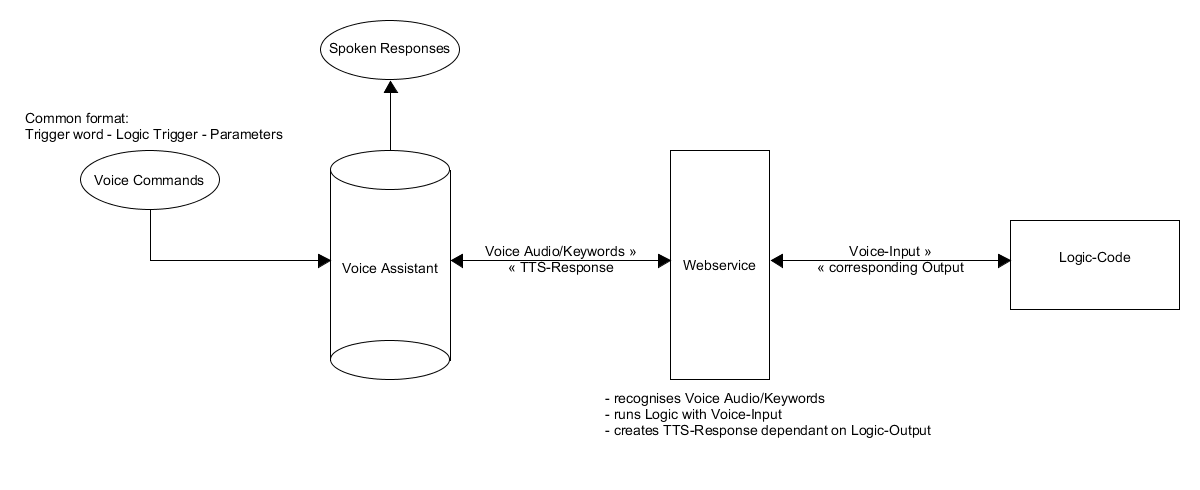
\includegraphics[scale=0.36]{content/img/GeneralVA_Architektur.png}
	\caption{Komponentendiagramm der generellen Funktionsweise eines Voice Assistants}
	\label{imgDiagramm}
\end{figure}

Wie in Abbildung \ref{imgDiagramm} beschrieben ist, muss der VA zunächst durch ein Trigger word aktiviert werden. Darauf folgt die so genannte Utterance. Diese setzt sich aus Logic Trigger und gegebenenfalls notwendigen Parametern zusammen. Diese wird mithilfe von SE auf dem Gerät erkannt und digitalisiert. Anschließend sendet der VA die Utterance an einen Webservice, der die weitere Verarbeitung übernimmt. So können die Voice Assistants schlank gehalten werden, da ein Großteil der Rechenarbeit auf dem Webservice erfolgt. \newline

Der Webservice erkennt nun anhand des Logic Triggers den konkreten Anwendungsfall und ermittelt, falls nötig, die gegebenen Parameter. Der konkrete Anwendungsfall wird als Intent bezeichnet. Die Anfrage wird daraufhin vom Webservice bearbeitet. Hierzu wird der auf einem Webserver abgelegten Logic-Code verwendet. Für jeden definierten Intent enthält der Logic-Code eine passende Funktion. Dies kann von einer einfachen Rechnung, über Suchanfragen im Internet bis hin zur Wiedergabe von akustischen Medien auf dem VA reichen.\newline

Der Logic-Code generiert eine zur Anfrage passenden Antwort, welche an den Webservice weitergereicht wird. Der Webservice erzeugt daraus eine TTS-Response, welche an den Voice Assistant gesendet wird. Letzterer ist nun in der Lage dem Anwender eine gesprochene Antwort auf seine Anfrage zu geben.

\subsection{Voice Assistant}
Im folgenden Schaubild wird veranschaulicht, was in Kapitel \ref{secOne} textuell beschrieben wird.
\begin{figure}[htb]
	\centering
	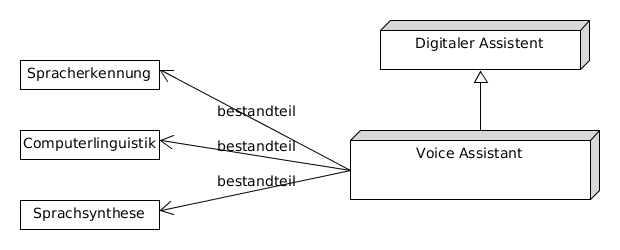
\includegraphics[scale=0.36]{content/img/bestandteile.png}
	\caption{Konzeptionelles Modell eines Voice Assistant}
	\label{imgBestandteile}
\end{figure}


\subsection{Webservice}
\subsection{Was ist ein Webservice?}
Ein Webservice erm\"{o}glicht eine Maschine-zu-Maschine Kommunikation mittels
HTTP oder HTTPS \"{u}ber das Internet. Auf einem entfernten Computer werden Funktionen
ausgef\"{u}hrt. Der Webservice wird mittels URI (Uniform Resource Identifier)
eindeutig identifiziert. Die Kommunikation kann HTTP, XML oder JSON basiert sein.

\subsection{Welchen Webservice nutzt Amazons Alexa?}
Alexa arbeitet mit dem Amazon Web Service (AWS). AWS ist ein Tochterunternehmen von Amazon.
AWS ist ein Cloud Computing Anbieter. Ein Nutzer von AWS bekommt einen virtuellen Server, welcher
auf einem echten Server innerhalb einer Serverfarm l\"{a}uft.
F\"{u}r diesen virutellen Server bietet AWS diverse Dienste an.
Die f\"{u}r den Voice Assistant ben\"{o}tigten sind dabei folgende:
\subsubsection{Lambda}
Der AWS Dienst Lambda f\"{u}hrt beliebigen Code auf dem virtuellen Server aus.
Meistens wird Lambda dazu verwendet eine Anfrage zu verarbeiten.
In dieser Anfrage wird eine Lambda Funktion aufgerufen, ein von einem Programmierer
entwickeltes Programm. Die Lambda Funktion generiert eine Antwort, meist im JSON-Format.
Zurzeit unterst\"{u}tzte Programmiersprachen mit den entsprechenden
Bibliotheken sind: Java, Node.js, Python und C\#.
In zusammenarbeit mit einem Voice Assistenten wird dem AWS Dienst Lambda eine Anfrage im
JSON-Format \"{u}bermittelt, in dieser steht die Lambda Funktion welche ausgef\"{u}hrt werden soll
mit eventuellen Parametern. Der hinterlegte Programmcode (Logic Code) wird ausgef\"{u}hrt.
Die Antwort im JSON-Format sendet AWS zur\"{u}ck an den Voice Assistant.
Dieser wandelt die Antwort mittels TTS in Sprache um und Antwortet dem Nutzer auf seine Anfrage.
\subsubsection{Alexa Voice Service (AVS)}
AVS versteht nat\"{u}rliche Sprache und kann diese in Text umwandeln.
Umgekehrt kann AVS Text wieder in Sprache umwandeln.
Die aktuellste Version des AVS wird von Alexa auf das Voice Assistant Ger\"{a}t heruntergeladen.
Der Voice Assistant wird dann lokal die Sprache in Text umwandeln und an den AWS senden.
Da AVS ein Teil der Amazon Web Services ist wird die Spracherkennung mittels Machine Learning
stettig verbessert, d.h. viele Ger\"{a}te senden erfolgreiche oder fehlgeschlagene Anfragen an AWS,
um die Spracherkennung zu verbessern. Durch das Alexa Skill Kit kann ein Entwickler dem AVS
zeigen welche Reaktion der Entwickler bei einem bestimmten Stichwort oder Satz erwartet.
Dabei muss nahezu jede m\"{o}gliche Variation des Satzes bedacht sein, damit entsprechend
darauf reagiert werden kann.

\subsection{Welchen Webservice nutzt Google Assistant?}
Die Google Home Ger\"{a}te integrieren den Google Assistant. Dieser kann mittels Dialogflow
(fr\"{u}her APi.ai) erweitert werden, wie vorher bereits mit mobilen Ger\"{a}ten oder dem Google Chrome
Browser m\"{o}glich. Dialogflow wird durch eine Node.js Node auf einem eigenen Server oder z.B.
einem Server des Google Cloud Projects ausgef\"{u}hrt. Der Entwickler hat einen Agent (Anwednung)
entwickelt, welcher auf die Anfrage des Nutzers reagiert.


\section{Alexa}
\label{secThree}
Alexa ist der Name eines von der Firma Amazon entwickelten Voice Assistenten. Die verschiedenen Gerätevarianten sind jeweils mit mindestens einem Lautsprecher und sieben Mikrofonen ausgestattet. In Deutschland werden diese Geräte seit dem 26. Oktober 2016 angeboten. Durch die Mikrofone nimmt das Gerät die Geräusche in der Umgebung auf und versucht daraus die menschliche Sprache herauszufiltern. Dadurch bieten die Geräte die Funktionen eines Digitalen-Assistenten mittels Spracherkennung an, auch genannt Voice Assistant.
Alexa reagiert nicht dauerhaft auf gesagt Textpassagen sondern erst sobald ein aus einer beschränkten Auswahl gewähltes Wort genannt wird. Hier bietet Amazons Alexa folgende Aktivierungswörter an: Alexa, Echo, Amazon oder Computer. Sollte eines der Aktivierungswörter genannt werden beginnt ein LED-Indikator blau zu leuchten. Alles nun gesagte wird zur Erkennung an die Alexa Voice Services gesendet, wodurch auch sensible Daten über das Internet übertragen werden. Lediglich das erste Wort wird lokal verarbeitet, auch bietet das Gerät einen fest verlöteten Schalter um das Mikrofon zu deaktivieren. Dies wird über einen roten LED-Indikator angezeigt.\\

\subsection{Funktionen/Funktionsweise}
Mit Beginn der Einrichtung, beherrscht der VA bereits grundlegende Dinge wie: Wecker,Erinnerungen,Wetter abfrage, Internetsuche,Musik abspielen etc. . Diese sind immer gleich Aufgebaut. Mit dem mitteilen des "WakeWords" (z.B. Alexa oder Computer) wird der VA aktiviert und dann kann mittels des anschließend gesprochenem Textes die entsprechende Aktion ausgeführt werden. Mit "Alexa, stell meinen Wecker auf 6:30 Uhr" spricht man den Wecker-Skill an. Es gibt mittlerweile über 10.000 Skills welche auch von vielen Drittanbietern entwickelt werden. Außerdem kann man mit Alexa auch über den Online-Store von Amazon einkaufen.

\begin{figure}[H]
	\centering
	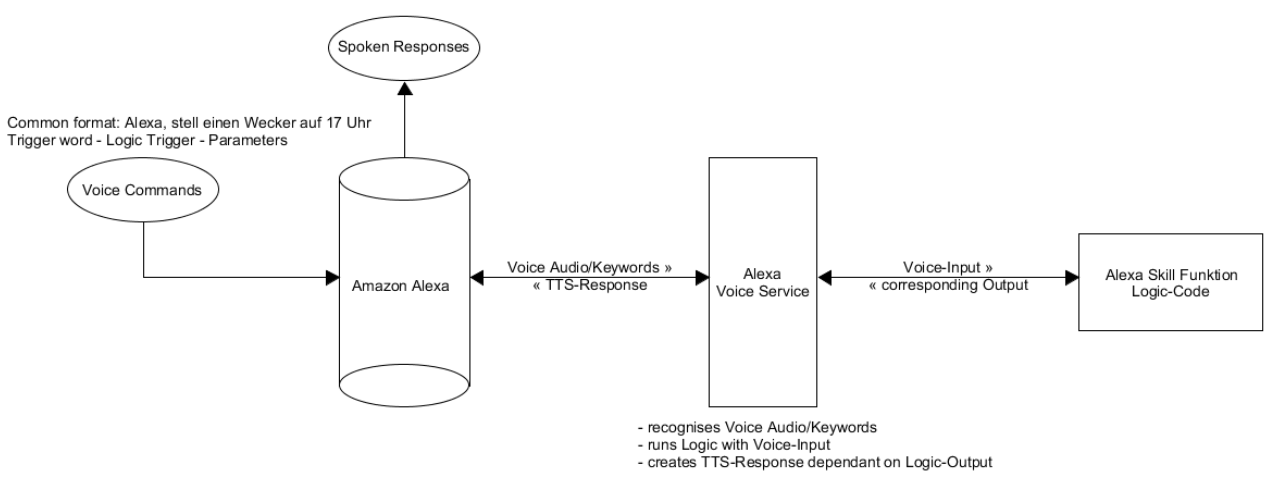
\includegraphics[width=0.9\textwidth]{content/img/AlexaVA_Architektur}
	\caption[Amazon Voice-Assistant Architektur]{Amazon Voice-Assistant Architektur}
\end{figure}

Oben wird die Struktur des VA als Diagramm gezeigt. Hier sieht man wie das Endgerät mit dem Alexa Voice Service kommuniziert und dieser dann alles entsprechend zusammenfügt und an die eigentliche Funktion übertragen. Diese verarbeitet dann die Abfrage und sendet eine Antwort zurück welche mittels TTS zu einer Stimme formatiert wird.

\subsection{Hardware}
Nachfolgend wird eine kleine Auswahl an Alexa-Geräten gezeigt. Insgesamt gibt es allerdings deutlich mehr.\\

Amazon Alexa Geräte:
\begin{itemize}
	\item Echo Spot (Alexa Lautsprecher mit kleinem Display)
	\item Echo Buttons ("Smart Home" Buttons)
	\item Echo Connect (Verbindet Alexa mit dem Telefon für Anrufe)
	\item Echo Show (7" Display - Anzeige von Videos und anderen Infos)
	\item Echo, Echo Dot und Echo Plus
	\item Alexa Sprachferbedienung (FireTV)
\end{itemize}

\subsubsection{Echo Dot (v2)}
\begin{figure}[H]
	\begin{minipage}{0.45\textwidth}
		\begin{itemize}
			\item 59,99€
			\item 7 Mikrofone - 1 Lautsprecher
			\item Hardwaretasten für die Lautstärke
			\item Arbeitet als Smart Home Hub
			\item ein Mute-Button für das Mikrofon auf dem Gerät
		\end{itemize}
	\end{minipage}
	\hfill
	\begin{minipage}{0.45\textwidth}
		\centering
		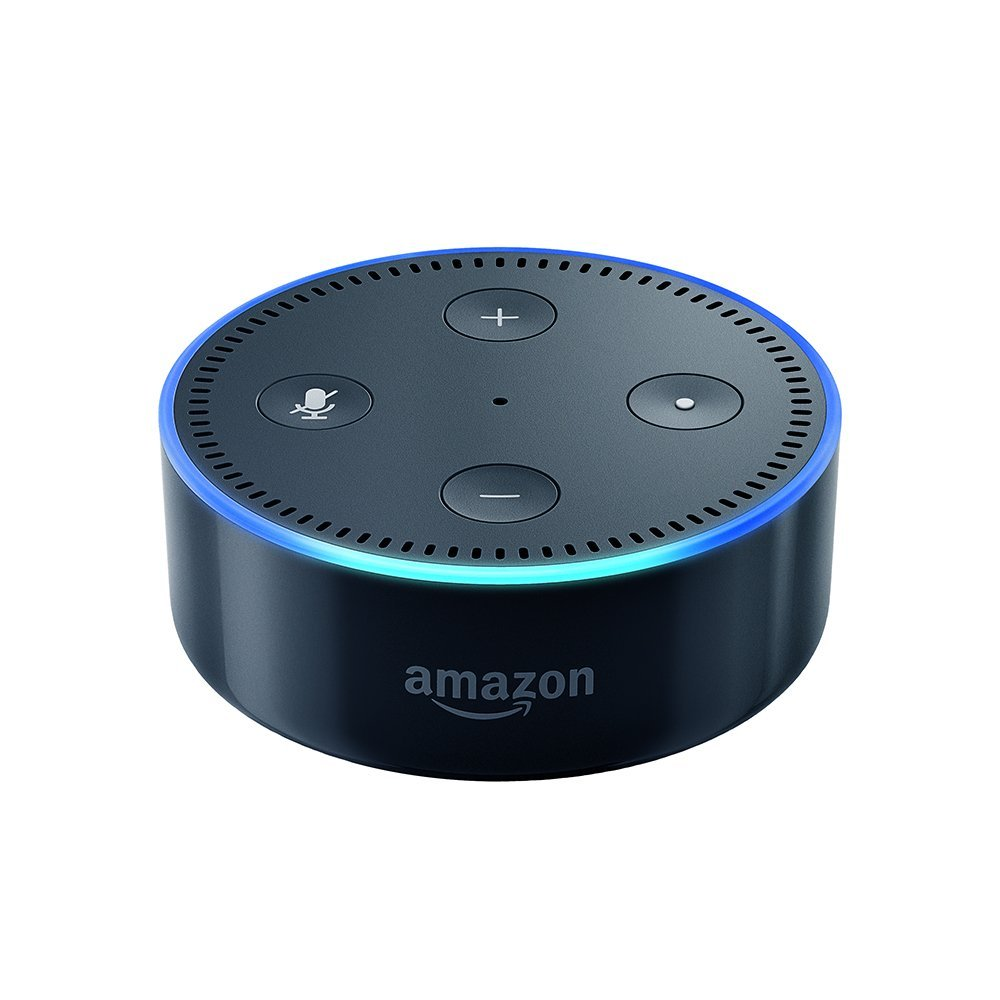
\includegraphics[width=\textwidth]{content/img/echodot}
		\caption[Echo Dot]{Echo Dot}
	\end{minipage}
\end{figure}

\subsubsection{Echo}
\begin{figure}[H]
	\begin{minipage}{0.45\textwidth}
		\begin{itemize}
			\item 99,99€
			\item Ähnlich wie Echo Dot
			\item Größere und bessere Lautsprecher
			\item 63mm-Woofer
			\item 16mm-Hochtonlautsprecher
		\end{itemize}
	\end{minipage}
	\hfill
	\begin{minipage}{0.45\textwidth}
		\centering
		
\includegraphics[width=\textwidth]{content/img/echo}
		\caption[Echo]{Echo}
	\end{minipage}
\end{figure}

\subsubsection{Echo Plus}
\begin{figure}[H]
	\begin{minipage}{0.45\textwidth}
		\begin{itemize}
			\item 149,99€
			\item Ähnlich wie Echo Dot und Echo
			\item integrierten ZigBee-Smart Home Hub
			\item Größere und bessere Lautsprecher
			\item 63mm-Woofer
			\item 20mm-Hochtonlautsprecher
		\end{itemize}
	\end{minipage}
	\hfill
	\begin{minipage}{0.45\textwidth}
		\centering
		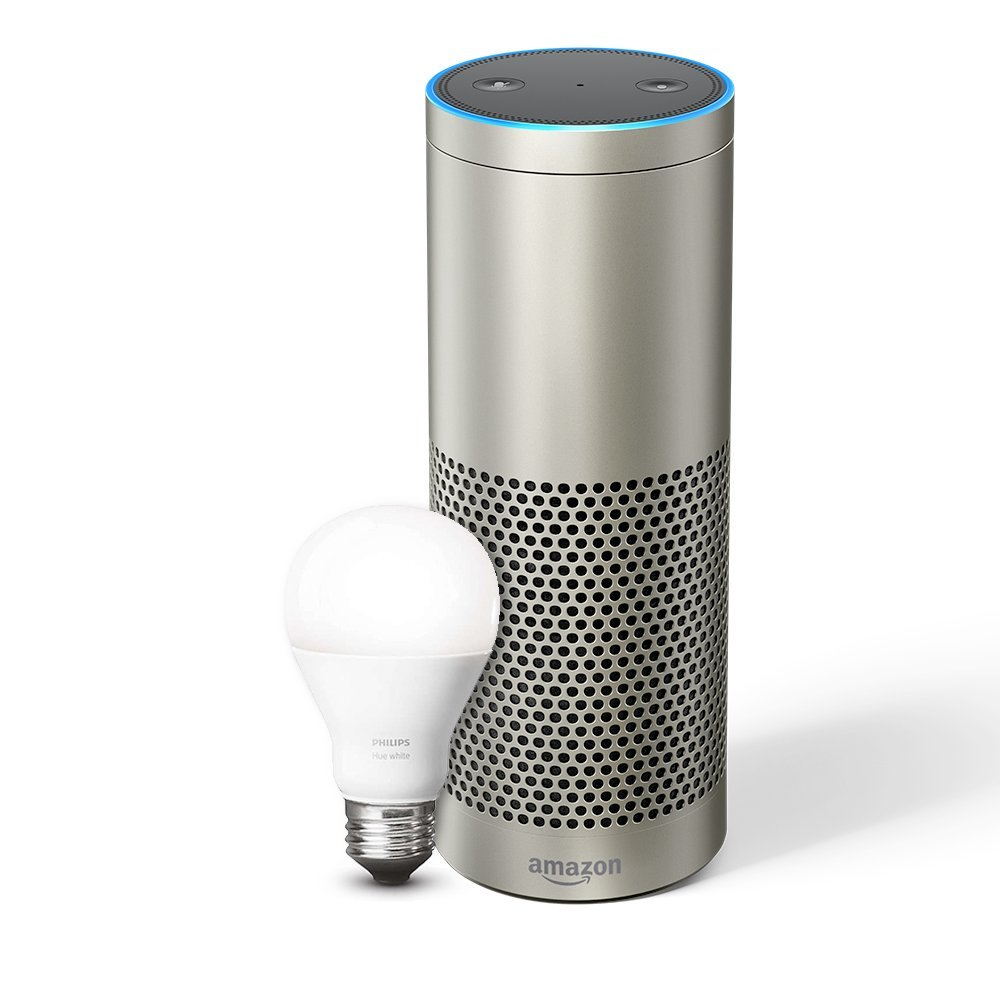
\includegraphics[width=\textwidth]{content/img/echoplus}
		\caption[Echo Plus]{Echo Plus}
	\end{minipage}
\end{figure}

\subsection{Erweiterbarkeit - Skills}
Der Alexa Skills Service bietet die Möglichkeit eigene Skills zu entwickeln und über den Store den anderen Nutzer bereitzustellen. Die Skills bedienen sich dabei einer Skills API, für welche es mittlerweile eine breite Unterstützung für viele verschiedene Programmier- und Skriptsprachen gibt. Jeder Skill verfolgt dabei ein festes Muster welches sich aus einem Dialogmuster, also einer Datei welche aussagt wie mit dem Nutzer kommuniziert wird und einer Funktion zusammensetzt. Diese Funktion wird in der Regel durch einen Webservice bereitgestellt, hierfür bietet sich der von Amazon bereitgestellte Service AWS Lambda an, da dieser bereits eine gute Integration in die Entwicklung darstellt.\\

Ein Skill besteht aus Utterances,Intents und einer Funktion. Utterances (auch Aussagen) werden einem Intent zugeordnet, der AVS nutzt diese um dem gesagten ein Intent zuzuweisen damit der korrekt Code ausgeführt wird. Ein paar Beispiele:
\begin{itemize}
	\item stell den Wecker
	\item wie spät ist es ?
	\item wann klingelt der Wecker ?
\end{itemize}
Diese zugeordneten Intents werden dann über einen eindeutigen Namen mit dem Code verknüpft. Im Code kann dann die entsprechende Antwort in Form eines Strings zurückgegeben werden.

\section{Google Home}
\label{secFour}

Google Home ist ein von Google entwickelter Smart-Home-Lautsprecher, der mit integriertem Mikrofon ausgestattet ist und über einen persönlichen Voice-Assistenten verfügt. Das Gerät wurde am 4. November 2016 in den Vereinigten Staaten veröffentlicht. In Deutschland erfolgte die Markteinführung am 8. August 2017 mit einer deutscher Stimme für den Voice-Assistenten.
Es gibt momentan drei verschiedene Google Home Geräte (Home, Home Mini, Home Max), die sich in erster Linie in ihrer Größe und der Qualität ihrer Lautsprecher unterscheiden.\\

\subsection{Funktionen/Funktionsweise}

Google Home kommt mit einer Reihe von Funktionen sowohl von Google als auch von Drittanbietern, die es dem Benutzer beispielsweise erlauben Musik zu hören, die Wiedergabe von Videos oder Fotos auf Smart-Home Geräten zu steuern oder aktuelle Nachrichten zu erhalten. Mehrere Google Home Geräte können in unterschiedlichen Räumen zum synchronisierten Abspielen von Musik verwendet werden. Ein Update im April 2017 ermöglicht es den Geräten bis zu sechs Benutzer anhand ihrer Stimme zu erkennen und individuell zu reagieren.\\
Um dem Gerät Befehle zu erteilen muss es zunächts mit den Weckworten ''\textit{Hey Google}'' oder ''\textit{Ok Google}'' aufgeweckt werden.
Um Drittanbietersoftware über die sogenannten Actions on Google zu nutzen ist keine Installation notwendig.\\
Der integrierte Google Assistant, den es auch außerhalb von Google Home Geräten (z.B. auf Android Smartphones) gibt, bietet dem Benutzer sein eigenes persönliches Google um ihm beim Suchen, Organisieren oder Interagieren zu helfen.\\
Actions on Google erweitert den Google Assistant um sogenannte Actions, die es Entwicklern ermöglicht eigene Funktionen hinzuzufügen. Anders als bei traditionellen mobilen oder Desktopapplikationen interagiert der Nutzer mit den Apps für den Assistenten über verbale Konversation (natürlich klingender Austausch zwischen Nutzer und App).\\
Ein typischer Ablauf eines solchen Austausches sieht wie folgt aus. Wenn ein Nutzer den Assistenten auffordert eine bestimmte Aktion auszuführen, sendet der Assistent eine Anfrage an Actions on Google um eine passende App zu finden, die der Intention des Nutzers entspricht.
Diese wird dann an den Assistenten weitergereicht und der Nutzer wird gefragt, ob er diese App ausführen möchte. Wenn der Nutzer dies bestätigt, wird die App vorgestellt und die Konversation an diese weitergereicht (siehe Abbildung 1).\\
\begin{figure}[H]
	\centering
	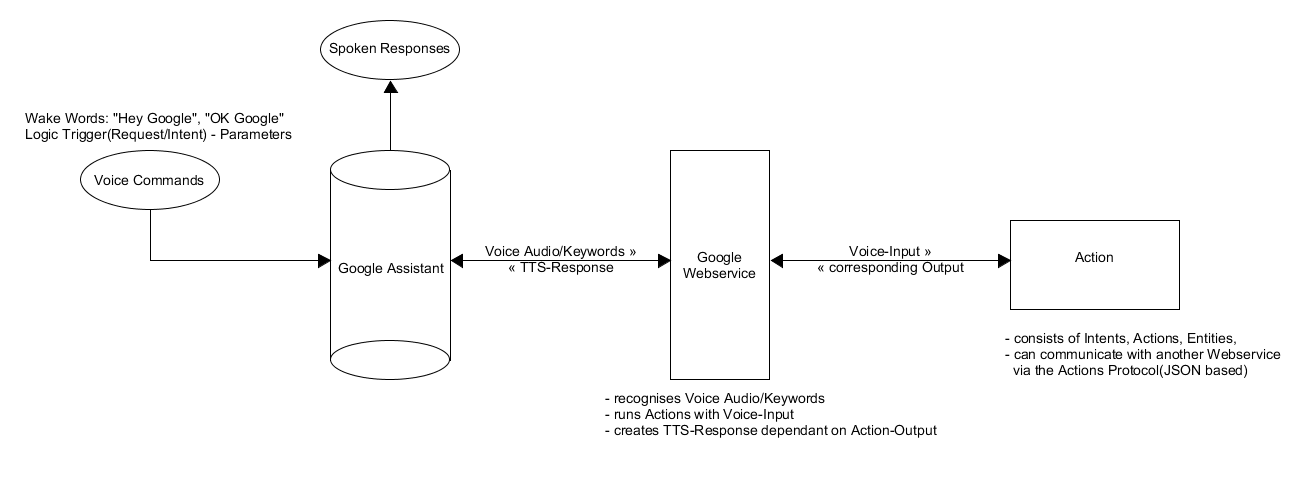
\includegraphics[width=0.9\textwidth]{content/img/GoogleVA_Architektur}
	\caption[Google Voice-Assistant Architektur]{Google Voice-Assistant Architektur}
\end{figure}
Der Google Assistant hat Zugriff auf Google Maps und kann daher Fragen zu Position örtlicher Geschäfte, sowie deren Öffnungszeiten beantworten. Generell steht dem Assistenten die Google Suche zur Verfügung um enzyklopedisches Wissen oder einfache Übersetzungen wiederzugeben.



\subsection{Hardware}

Es folgt ein kurzer Überblick über die verschiedenen Google Home Geräte, die momentan im Handel erhältlich sind.

\subsubsection{Google Home}
\begin{figure}[H]
	\begin{minipage}{0.45\textwidth}
	  \begin{itemize}
	  \item 149€
	  \item farbige Status-LEDs an der Oberfläche
	  \item kapazitiver Berührungssensor um Musik zu starten und stoppen oder die Lautstärke anzupassen
	  \item ein Mute-Button für das Mikrofon an der Rückseite
	  \end{itemize}
	\end{minipage}
	\hfill
	\begin{minipage}{0.45\textwidth}
	  \centering
	  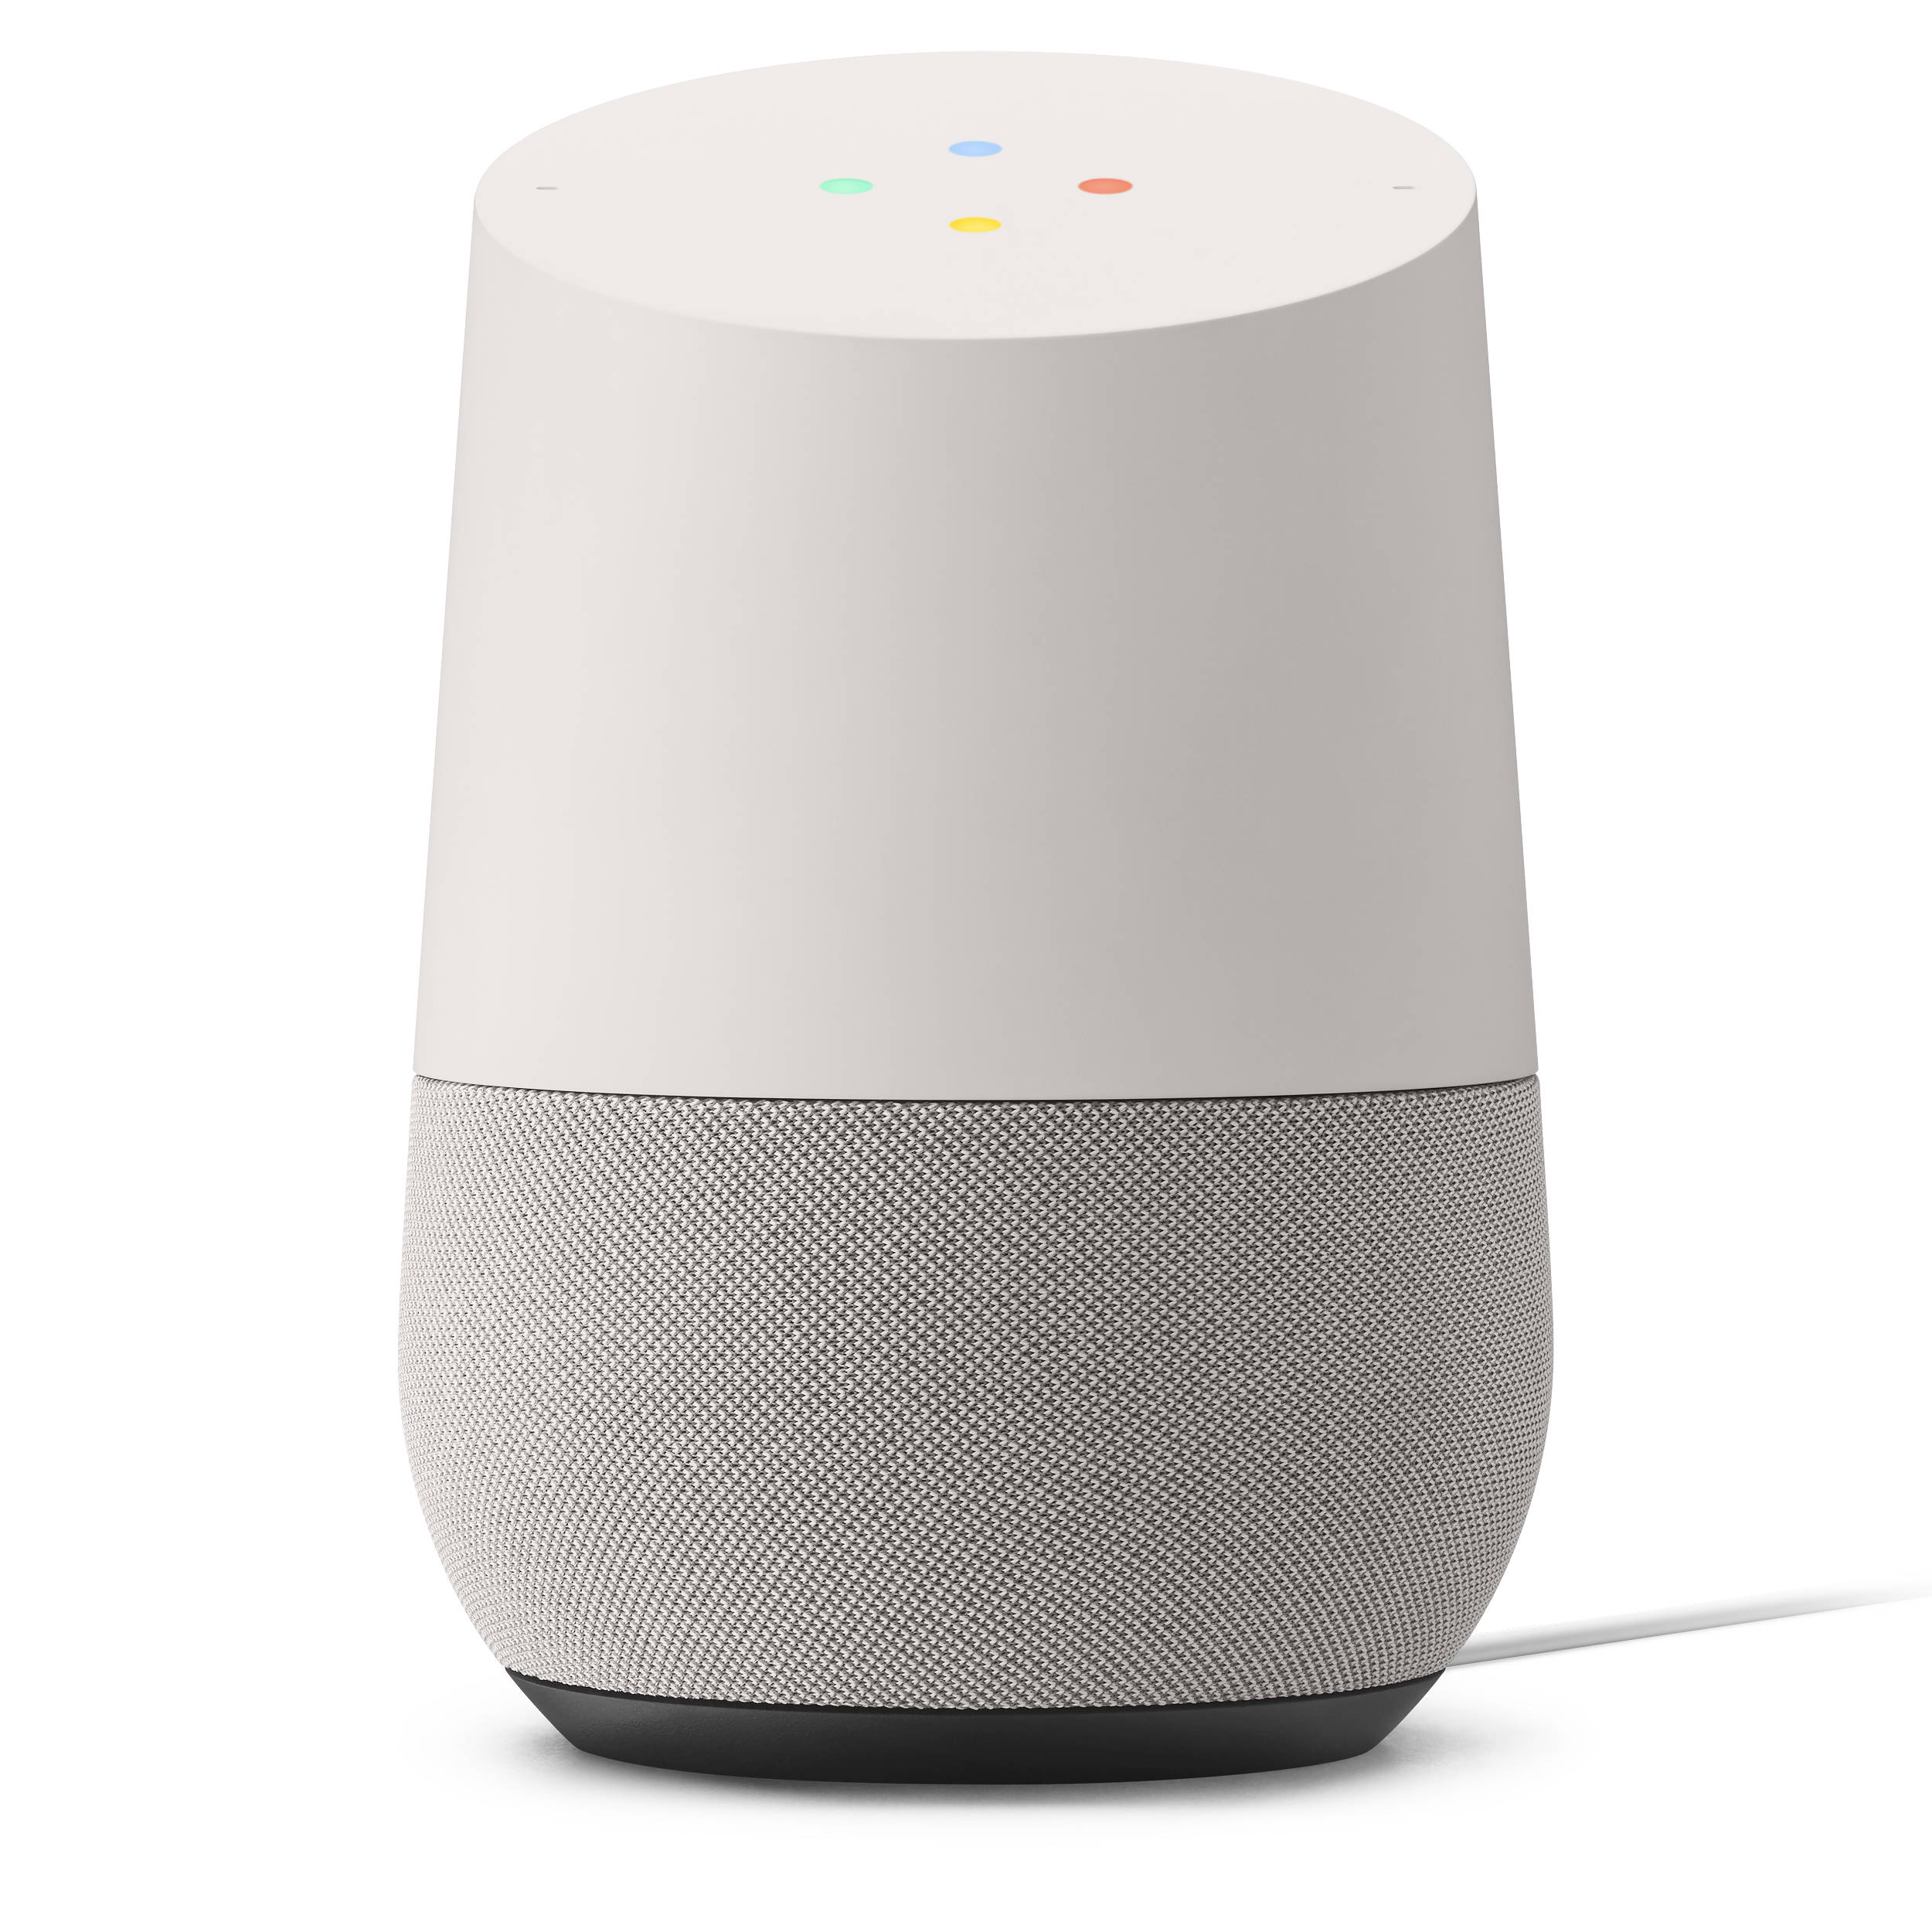
\includegraphics[width=\textwidth]{content/img/GoogleHome}
	  \caption[Google Home]{Google Home}
	\end{minipage}
\end{figure}

\subsubsection{Google Home Mini}
\begin{figure}[H]
	\begin{minipage}{0.45\textwidth}
	  \begin{itemize}
	  \item 59€
	  \item gleiche Funktionalität
	  \item Berührungssensor zum Anpassen der Lautstärke
	  \item weiße Statuslichter scheinen durch den Stoff auf der Oberseite
	  \item ein Mute-Schalter für das Mikrofon an der Rückseite
	  \end{itemize}
	\end{minipage}
	\hfill
	\begin{minipage}{0.45\textwidth}
	  \centering
      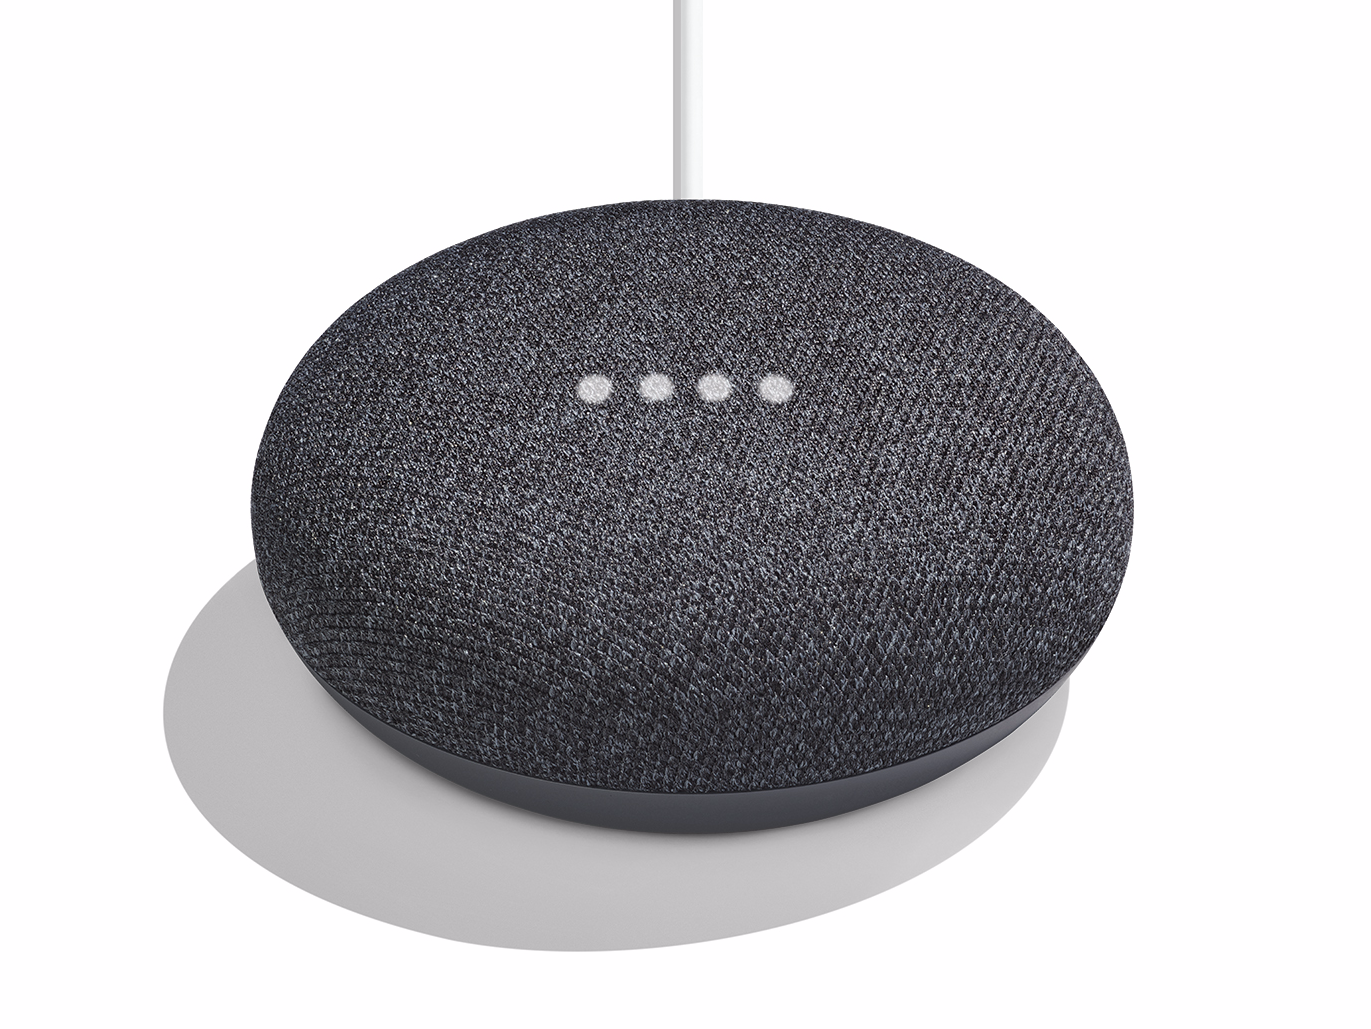
\includegraphics[width=\textwidth]{content/img/GoogleHomeMini}
      \caption[Google Home Mini]{Google Home Mini}
	\end{minipage}
\end{figure}

\subsubsection{Google Home Max}
\begin{figure}[H]
	\begin{minipage}{0.45\textwidth}
	  \begin{itemize}
	  \item 400\$
	  \item Stereo Lautsprecher(einschließlich zweier Hochtöner und Subwoofer)
	  \item magnetisch befestigbarer Ständer für vertikale Ausrichtung
	  \item beinhaltet \textit{Smart Sound}, ein Soundsystem das \textit{machine learning} nutzt um sich automatisch an die Umgebung anzupassen(Position und Geräuschquellen)
	  \end{itemize}
	\end{minipage}
	\hfill
	\begin{minipage}{0.45\textwidth}
	  \centering
      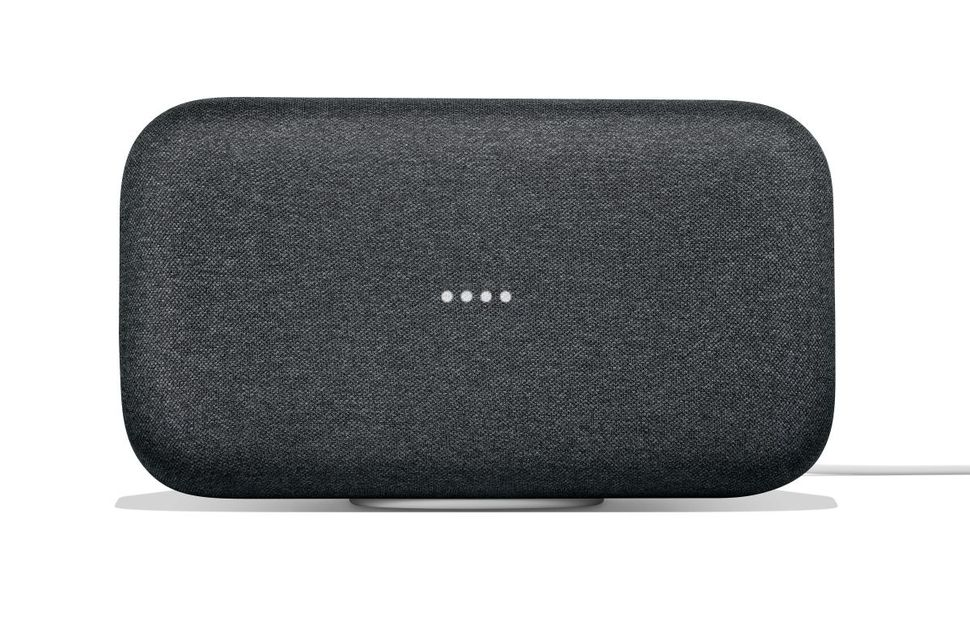
\includegraphics[width=\textwidth]{content/img/GoogleHomeMax}
      \caption[Google Home Max]{Google Home Max}
	\end{minipage}
\end{figure}

\subsection{Erweiterbarkeit}

Um eine App für den Google Assistant zu entwickeln bietet Google verschiedene Optionen.
Zum einen gibt es Templates, die einem einen Großteil der Programmierarbeit abnehmen und bereits vorgefertigte Konversationen enthalten. Allerdings gibt es bisher nicht viele Templates aus denen man wählen kann.\\
Für einfache Apps mit wenig Inputmöglichkeiten bietet sich die \textit{Actions SDK} an. Sie bietet keine NLU (natural language understanding), es kann allerdings eine eigene NLU eigesetzt werden.
Weiterhin müssen \textit{action packages} mit einem Text Editor geschrieben und per Kommando-Zeilen Tool an das jeweilige Google Developer Projekt gesendet werden.\\
\textit{Dialogflow} ist eine Web IDE, die die Funktionalität der \textit{Actions SDK} einschließt.
\textit{Dialogflow} beinhaltet eine \textit{NLU engine} die natürliche, menschliche Sprache parsen kann.

\subsection{Actions}

Im Folgenden wird auf den Aufbau der Actions in Dialogflow eingegangen.\\
Intents sind ein Hauptbestandteil der Actions. Sie werden mithilfe von \textit{machine learning} von Dialogflow aus \textit{Utterances} (Äußerungen des Nutzers) bestimmt. Die Intents können mehrere Parameter enthalten. Diese können von der \textit{NLU engine} als Entities erkannt werden.\\
Entities sind Tabellen in denen Einträge von Objekten eines Typs vordefiniert werden können.
Zur Unterstützung der Spracherkennung können Synonyme für die Objekte eigetragen werden.
Sie dienen zur Erkennung von relevanten Daten in den Intents.\\
Als Antwort auf ein Intent kann eine Text Response zurückgegeben werden. Unter dem Menüpunkt Fullfilment kann allerdings auch auf einen Webservice verlinkt werden, an den geparste Intents über das \textit{Actions Protocol} (JSON basiert) versendet werden. Der Webservice kann daraufhin den Inhalt auswerten und eine Antwort zurücksenden, die dann von der Action zurückgegeben werden kann.

%%%%%%%%%%%%%%%%%% Ende des Dokuments %%%%%%%%%%%%%%%%%%%%%


\end{document}
%% Dokument ENDE %%%%%%%%%%%%%%%%%%%%%%%%%%%%%%%%%%%%%%%%%%%%%%%%%%%%%%%%%%

